\smartdiagramset{%
  back arrow disabled=true,
  module minimum width=2cm,
  module minimum height=2cm,
  module x sep=3cm,
  text width=2cm,
  additions={
    additional item offset=0.5cm,
    additional item border color=red,
    additional arrow color=red,
    additional item width=2cm,
    additional item height=2cm,
    additional item text width=3cm
  }
}

\begin{figure}[h]
  \centering
  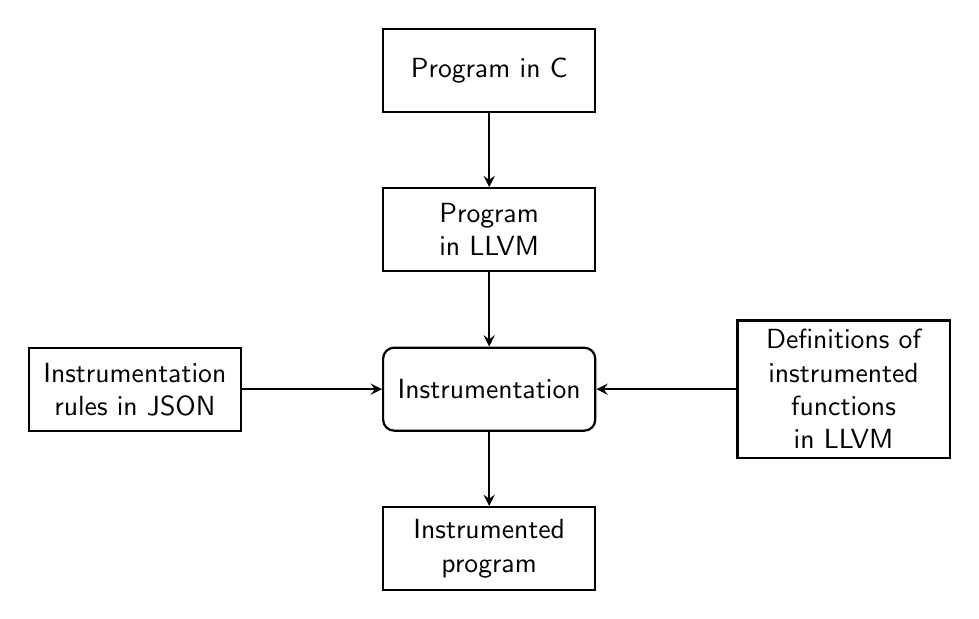
\begin{tikzpicture}[yscale=0.9, auto,
      block/.style = {
        rectangle, draw=black, thick, text width=7em, text centered,
        rounded corners, minimum height=3em },
      block-sharp/.style = {
          rectangle, draw, thick, text width=7em, text centered, minimum
          height=3em },
      line/.style = { draw, thick, ->, >=stealth },
      line-dashed/.style = { draw, thick, ->, densely dotted, >=stealth }]
    \node [block-sharp] (rules) at (-4.5, -2.25) {\textsf{Instrumentation\\ rules in JSON}};
    \node [block-sharp] (cprogram) at (0, 2.25) {\textsf{Program in C}};
    \node [block-sharp] (llvmprogram) at (0, 0) {\textsf{Program in LLVM}};
    \node [block] (instr) at (0, -2.25) {\textsf{Instrumentation}};
    \node [block-sharp] (instrprogram) at (0, -4.5) {\textsf{Instrumented program}};
    \node [block-sharp] (defs) at (4.5, -2.25) {\textsf{Definitions of
    instrumented functions in LLVM}};
    % connect all nodes defined above
    \draw[line] (cprogram) -> (llvmprogram);
    \draw[line] (llvmprogram) -> (instr);
    \draw[line] (instr) -> (instrprogram);
    \draw[line] (rules) -> (instr);
    \draw[line] (defs) -> (instr);
  \end{tikzpicture}
  \caption{The scheme of Configurable Instrumentation.}
  \label{fig:scheme}
\end{figure}

The basic idea of our instrumentation tool is depicted in
figure~\ref{fig:scheme}. Since it works on LLVM, a program in C that is
supposed to be instrumented has to be translated. Instrumentation is required
to be configurable, therefore it needs to be supplied with two files: a file
with definitons of instrumentation functions whose calls will be inserted into
the code and a JSON file with instrumentation rules. The rules define how
sequences of LLVM instructions should be instrumented with calls of
instrumentation functions. The tool first loads a whole module from a given
LLVM code and begins to process it. In each phase it goes through all functions
and it first applies rules for inserting instructions at their entry points and
above their terminator instructions. Then it goes through instructions of the
current function and it looks if they match with the sequences described in
instrumentation rules. If a match is found, the current sequence of
instructions is instrumented above or under according to the instrumentation
rules. At the very end, a rule for global variables is applied. The result of
the instrumentation process is again an LLVM program.

\section{Conditions}\label{sec:conditions}

To enable conditional instrumentation, the rules can contain conditions. A
condition is a conjunction of predicates over values from the program.
\todo{describe later when we solve the issue with condition system}

\section{Flags}
In order to pass some information between phases, flags can be defined in a
JSON file with instrumentation rules. When inserting a call to a function, it
is possible to set a flag and in a later phase condition some rule by a check
whether the flag is set to some value.

\section{Plugins}

The instrumentation module can be extended by plugins that can reply to queries
derived from conditions belonging to rules. Since static analyses provided by
plugins are supposed to be over-approximating, the predicates are set to reason
about possibilities (e.g. may the pointer be invalid?). Therefore answering
true is a conservative answer if an analysis does not have enough information
to refute the predicate. A condition is evaluated as \emph{true} if all plugins
answer that it is satisfied. If at least one plugin says that the condition is
not satisfied, the condition is evaluated as \emph{false}.

To define a list of possible conditions, all plugins have to implement the same
interface.
\todo{describe interface and how it works}

\section{Configuration}

\lstset{
    basicstyle=\footnotesize,
    string=[s]{"}{"},
    stringstyle=\color{blue},
    comment=[l]{:},
    commentstyle=\color{black},
}

\begin{figure}[h]
\lstinputlisting{examples/json_example.json}
\caption{Example of an \texttt{instructionRule} in a JSON configuration file.}
\label{fig:json_example}
\end{figure}

\begin{figure}[h]
\lstinputlisting{examples/json_example2.json}
\caption{Example of an \texttt{globalVariablesRule} in a JSON configuration file.}
\label{fig:json_example2}
\end{figure}

The JSON file contains following fields:

\medskip
\begin{itemize}
\item \texttt{file:} Path to a a file with definitions of instrumentation functions.
\item \texttt{analyses:} List of paths to analyses plugins.
\item \texttt{flags:} List of flags that can be set during instrumentation.
\item \texttt{phases:} List of instrumentation phases. Each phase contains a
  list of \texttt{instructionRules}. Each rule is described with several fields:
  \begin{itemize}
    \item \texttt{findInstructions}: Sequence of instructions we are searching
    for. For each instruction in the sequence, we need to fill in an
        \texttt{instruction} field, that specifies a name of the instruction,
        \texttt{returnValue} that enables to remember the return value of the
        instruction in a given variable (can be set to "*" if the return value
        is not needed), and \texttt{operands} that enables either to match the
        operands or to remember the operand values in given variables. We can
        also optionally fill in fields \texttt{getSizeTo} and
        \texttt{getPointerInfoTo}. \texttt{getSizeTo} can be used only with
        \texttt{load}, \texttt{store} or \texttt{alloca} instruction and it
        stores size of the type of the value that is being loaded, stored or
        allocated to the given variable. \texttt{getPointerInfoTo} can be used
        only with \texttt{load} or \texttt{store} and it stores two values to
        given variables (if possible): size of the allocated memory to which
        the dereferenced pointer points to and corresponding \texttt{alloca}
        instruction. Since we can get this information only from a pointer
        analysis, this field can be used only when the analysis is available as
        a plugin.
    \item \texttt{newIstruction:} Instruction that is to be inserted. It
    contains two mandatory fields: \texttt{instruction} that specifies a name
    of the new instruction (for now, only \texttt{call} instruction is
    supported), and \texttt{operands} of the instruction.
    \item \texttt{in:} Name of a function, in which this rule should be
    applied. Can be set to a value "*" meaning that it should be used in all
    functions.
    \item \texttt{where:} Specifies the location of insertion. It can be:
      \texttt{before} or \texttt{after} the found sequence of instructions,
      \texttt{entry} (at the entry point of the given function, \texttt{in}
      cannot be set to "*" in this case) or \texttt{return} (before every
      terminator instruction of the given function, \texttt{in} cannot be set to
      "*" in this case).
    \item \texttt{setFlags:} List of pairs \texttt{<flag, value>} that sets
      all \texttt{flags} to a corresponding \texttt{value} if the rule was
      applied. This field is optional.
    \item \texttt{conditions:} List of conditions that have to be satisfied
    (see section~\ref{sec:conditions}). Conditions are lists where the first
    element is a name of a condition and other elements are parameters passed
    to the condition.
  \end{itemize}
\item \texttt{globalVariablesRule:} A rule for instrumenting global
  variables. The rule is described with several fields:
  \begin{itemize}
    \item \texttt{findGlobals:} Contains one mandatory field
    \texttt{globalVariable} that stores a value of a global variable to the
    given variable, and one optionall field \texttt{getSizeTo} that gets the
    size of the type of the global variable.
    \item \texttt{newInstruction:} The same as in \texttt{instructionRule}.
    \item \texttt{in:} Name of a function, at the beginning of which the rule
    should be applied.
    \item \texttt{conditions:} The same as in \texttt{instructionRule}.

  \end{itemize}

\end{itemize}

In figure~\ref{fig:json_example}, we can see an example of an
\texttt{instructionRule}. In this case, every time the tool comes across a
\texttt{load} instruction in any function (\texttt{in} is set to "*"), the only
operands of \texttt{load} is stored to a variable \texttt{<t1>}, size of the
type that is being load is stored to a variable \texttt{<t2>} and condition
\texttt{!isValidPointer} is checked (i.e. a plugin's function
\texttt{isValidPointer} is called with arguments \texttt{<t1>} and
\texttt{<t2>}). If the condition holds, call of a function
\texttt{\_\_INSTR\_check\_pointer} with arguments \texttt{<t1>} and
\texttt{<t2>} is inserted \emph{before} the current \texttt{load} instruction.
After a successful application of this rule, flag \texttt{loadPresent} is set
to \emph{true}.

An example of a \texttt{globalVariablesRule} can be found in
figure~\ref{fig:json_example2}. The value of a global variable is stored to a
variable \texttt{<t1>} and size of the type of the global variable is stored to
a variable \texttt{<t2>}. A plugin is asked whether the given condition
\texttt{isRemembered} with argument \texttt{<t1>} holds and if the answer is
positive, new call of a function \texttt{\_\_INSTR\_remember\_global} with
arguments \texttt{<t1>} and \texttt{<t2>} is inserted at the beginning of
\emph{main}.

The functions whose calls are instrumented into a code must be defined in a
file specified by the \texttt{file} field in the JSON configuration. This file
has to be compiled to LLVM and after a successful instrumentation, the
definitions of functions must be linked to the instrumented module.
